\documentclass[12pt,a4paper]{article}
\usepackage[14pt]{extsizes}
\usepackage[utf8]{inputenc}
\usepackage{amsfonts}
\usepackage{amssymb}
\usepackage{cmap}
% for fonts
    \usepackage[T2A, T1]{fontenc}
    \usepackage[english, russian]{babel}
    \usepackage{fontspec}
    \defaultfontfeatures{Ligatures=TeX,Renderer=Basic}
    \setmainfont[Ligatures={TeX, Historic}]{Times New Roman}
    \setsansfont{Times New Roman}
    \setmonofont{Courier New}
%plot
%mathcha.io
\usepackage{amsmath}
\usepackage{tikz}
\usepackage{mathdots}
\usepackage{yhmath}
\usepackage{cancel}
\usepackage{color}
\usepackage{siunitx}
\usepackage{array}
\usepackage{multirow}
\usepackage{amssymb}
\usepackage{gensymb}
\usepackage{tabularx}
\usepackage{booktabs}
\usetikzlibrary{fadings}
%mathcha.io
\usepackage{mathrsfs}
\usetikzlibrary{arrows}
\pagestyle{empty}
%plot
\usepackage{float}% for \begin{figure}[H]
\usepackage{cases}
\usepackage{graphicx}
\usepackage[left=2cm,right=2cm,top=2cm,bottom=2cm]{geometry}
\author{Аверьянов Тимофей, Корякин Алексей}
\begin{document}
\begin{center}
\textbf{Лекция №2:}

{\large Модель поведения потребителя}

\textbf{План}
\end{center}

\begin{enumerate}
\item Модель способности потребителя сопоставлять наборы благ;
\item Безразличные наборы благ и множества безразличия (кривые безразличия);
\item Теорема Жерар Дебре и функция полезности потребителя;
\item Модель Маршалла-Вальраса поведения потребителя на рынке благ.
\end{enumerate}





Занумеруем натуральными числами $\displaystyle 1,\ 2,\ \cdots ,n$ те виды благ, которые интересуют потребителя. Различные наборы данных благ мы будем обозначать $\displaystyle \vec{x}^{( 1)}$ и $\displaystyle \vec{x}^{( 2)}$.


\begin{equation*}
\vec{x}^{*} =\left( x^{*}_{1} ,\ x^{*}_{2} ,\cdots ,\ x^{*}_{n}\right) \ \in R^{+}_{n} \ =C \eqno(1)
\end{equation*}
\begin{equation*}
\begin{cases}
\vec{x}^{( 1)} =\left( x^{( 1)}_{1} ,\ x^{( 1)}_{2} ,\cdots ,\ x^{( 1)}_{n}\right) \ \in R^{+}_{n} \ =C\\
\vec{x}^{( 2)} =\left( x^{( 2)}_{1} ,\ x^{( 2)}_{2} ,\cdots ,\ x^{( 2)}_{n}\right) \ \in R^{+}_{n} \ =C
\end{cases}
\eqno(2)
\end{equation*}


Зададимся вопросом почему потребитель предпочитает например набор $\displaystyle \vec{x}^{( 1)}$ набору $\displaystyle \vec{x}^{( 2)}$. Это означает, что потребитель умеет сопоставлять любые два набора благ и в итоге сопаставления давать себе отчёт какой из этих наборов предпочтительней. Сделанный выше вывод мы оформим ввиде следующей модели способности потребителя. Потребитель сопоставляя наборы $\displaystyle \vec{x}^{( 1)}$, $\displaystyle \vec{x}^{( 2)}$ приходит к одному из двух выводов:
\begin{enumerate}
\item $\displaystyle A\ =\ \vec{x}^{( 1)}$ не хуже чем $\displaystyle \vec{x}^{( 2)}$
\item $\displaystyle \overline{A} \ =\ \vec{x}^{( 1)}$хуже $\displaystyle \vec{x}^{( 2)}$
\end{enumerate}
\begin{equation*}
wpr\ \left(\vec{x}^{( 1)} ,\vec{x}^{( 2)}\right) =\ \begin{cases}
A\ =\ \left(\vec{x}^{( 1)} \ не\ хуже\ чем\ \vec{x}^{( 2)}\right)\\
\overline{A} \ =\ \left(\vec{x}^{( 1)} хуже\ \vec{x}^{( 2)}\right)
\end{cases}
\eqno(3)
\end{equation*}
В итоге сопоставления потребитель делает одно из следующий утверждений. В математике функции двух элементов называются бинарными отношениями и областью определения таких функций служит декартово произведение $\displaystyle C^{2}$ просто благ. Множеством изменения такой функции такого бинарного отношения является набор из двух словестных альтернатив $\displaystyle \left( A,\ \overline{A}\right)$.
\begin{equation*}
wpr:C^{2} \ \rightarrow \left( A,\ \overline{A}\right) \eqno(4)
\end{equation*}
\begin{center}

\textbf{Две аксиомы функции }$\displaystyle wpr$
\end{center}

\begin{enumerate}
\item Аксиома транзитивности. Пусть $\displaystyle \vec{x}^{( 1)}$ не хуже чем $\displaystyle \vec{x}^{( 2)}$, а $\displaystyle \vec{x}^{( 2)}$ предпочительнее $\displaystyle \vec{x}^{( 3)}$, тогда $\displaystyle \vec{x}^{( 1)}$ набор предпочтительнее $\displaystyle \vec{x}^{( 3)}$:
\begin{equation*}
\begin{cases}
wpr\ \left(\vec{x}^{( 1)} ,\vec{x}^{( 2)}\right) \ =A,\\
wpr\ \left(\vec{x}^{( 2)} ,\vec{x}^{( 3)}\right) \ =A
\end{cases} \Rightarrow wpr\ \left(\vec{x}^{( 1)} ,\vec{x}^{( 3)}\right) =\ A. \eqno(5)
\end{equation*}
\item Аксиома не насыщаемости. Пусть каждая компонента в $\displaystyle \vec{x}^{( 1)}$ не меньше соотвествующей компоненты $\displaystyle \vec{x}^{( 2)}$. Тогда $\displaystyle \vec{x}^{(1)} \ \geq \vec{x}^{( 2)} \ \rightleftarrows \vec{x}^{( 1)}_{i} \ \geq \vec{x}^{( 2)}_{i} \ \text{при} \ \forall i\ \rightarrow \vec{x}^{( 1)} \succeq \ \vec{x}^{( 2)}$.
   Полагаем, что потребитель обладает свойством $\displaystyle wpr$ сопоставлять любые два набора благ, и это свойство удовлетворяет двум аксиомам тарнзитивности и ненасыщаемости.
\end{enumerate}
\begin{center}
\textbf{Безразличные наборы благ}
\end{center}
Если из двух наборов $\displaystyle \vec{x}^{( 1)}$ и $\displaystyle \vec{x}^{( 2)}$ потребитель не может выбрать предпочтительный для него набор благ, \ то такие наборы называются \textit{безразличными. }Вот определение:
\begin{equation*}
\begin{cases}
wpr\ \left(\vec{x}^{( 1)} ,\vec{x}^{( 2)}\right) \ =A,\\
wpr\ \left(\vec{x}^{( 2)} ,\vec{x}^{( 1)}\right) \ =A
\end{cases} \Rightarrow \vec{x}^{( 1)} \sim \vec{x}^{( 2)} .
\eqno(6)
\end{equation*}
Тогда такие наборы называются безразличными и обозначаются символом $\displaystyle \sim $.

Пусть $\displaystyle \vec{x}$некоторый набор благ. Множеством безразличия называют все наборы благ $\displaystyle \vec{y}$ каждый из которых безразличен набору $\displaystyle \vec{x}$.
\begin{equation*}
I\left(\vec{x}\right) \ =\ \left(\vec{y} |\vec{y} \ \in C,\ \vec{y} \ \sim \vec{x}\right) \eqno(7)
\end{equation*}
В ситуации двух благ множество безразличия на графике представляет собой кривую линию и называется\textit{ кривой безразличия.} Добавим к сказанному, что $\displaystyle wpr$ пораждает отношение безразличия, которое определено соотношением (8). Значение функции $\displaystyle rin$ на любых двух наборах благ $\displaystyle \left(\vec{x}^{( 1)} ,\vec{x}^{( 2)}\right)$ равно либо альтернативе $\displaystyle B$, либо $\displaystyle \overline{B}$. $\displaystyle B$ обозначает, что набор $\displaystyle \vec{x}^{( 1)}$ безразличен набору $\displaystyle \vec{x}^{( 2)}$. В математике функции с определением (8) носят отношение эквивалентности.


\begin{equation*}
rin\ \left(\vec{x}^{( 1)} ,\vec{x}^{( 2)}\right) =\ \begin{cases}
\vec{x}^{( 1)} \sim \vec{x}^{( 2)} =B,\\
\overline{B} .
\end{cases}
\eqno(8)
\end{equation*}
Теорема.
\begin{enumerate}
\item Если $\displaystyle rin\ \left(\vec{x}^{( 1)} ,\vec{x}^{( 2)}\right) \ =\overline{B} ,\ то\ I\left(\vec{x}^{( 1)}\right) \ \cap I\left(\vec{x}^{( 2)}\right) =\emptyset .$
\end{enumerate}

Теорема Дебре. Если $\displaystyle wpr$ транзитивно, непрерывно, удовлетворяет аксиомам ненасыщенности и выпуклости, то существует непрерывная на $\displaystyle C$ скалярная функция $\displaystyle u\left(\vec{x}\right)$, возрастающаяпо каждому аргументу и выпуклая вврех, такая, что


\begin{gather*}
если\ wpr\ \left(\vec{x}^{( 1)} ,\vec{x}^{( 2)}\right) \ =A,\ то\ \\
\ u\left(\vec{x}^{( 1)}\right) \ \geq u\left(\vec{x}^{( 2)}\right)
\end{gather*}
То есть если $\displaystyle \vec{x}^{( 1)} предпочтительнее\ \vec{x}^{( 2)}$, то на наборе $\displaystyle \vec{x}^{( 1)}$ $\displaystyle u\left(\vec{x}^{( 1)}\right) \ \geq u\left(\vec{x}^{( 2)}\right)$.

Экономисты пользуются следующими примерами функции полезности:
\begin{itemize}
\item Неоклассическая функция полезности $\displaystyle a_{0} \ \cdot \ x^{a_{1}}_{1} \ \cdot \ x^{a_{2}}_{2} \ \cdot \ \cdots \cdot \ x^{a_{n}}_{n}$
\item Логарими Бернулли $\displaystyle u\ =\ a_{1} \ \ln( x_{1} \ -\ c_{1}) \ +\ a_{2} \ \ln( x_{2} \ -c_{2}) \ +\ a_{n} \ \ln( x_{n} \ -c_{n})$.
\end{itemize}

Отметим график неокласической функции полезности графика двух граф:

\begin{center}
\begin{figure}[H]
  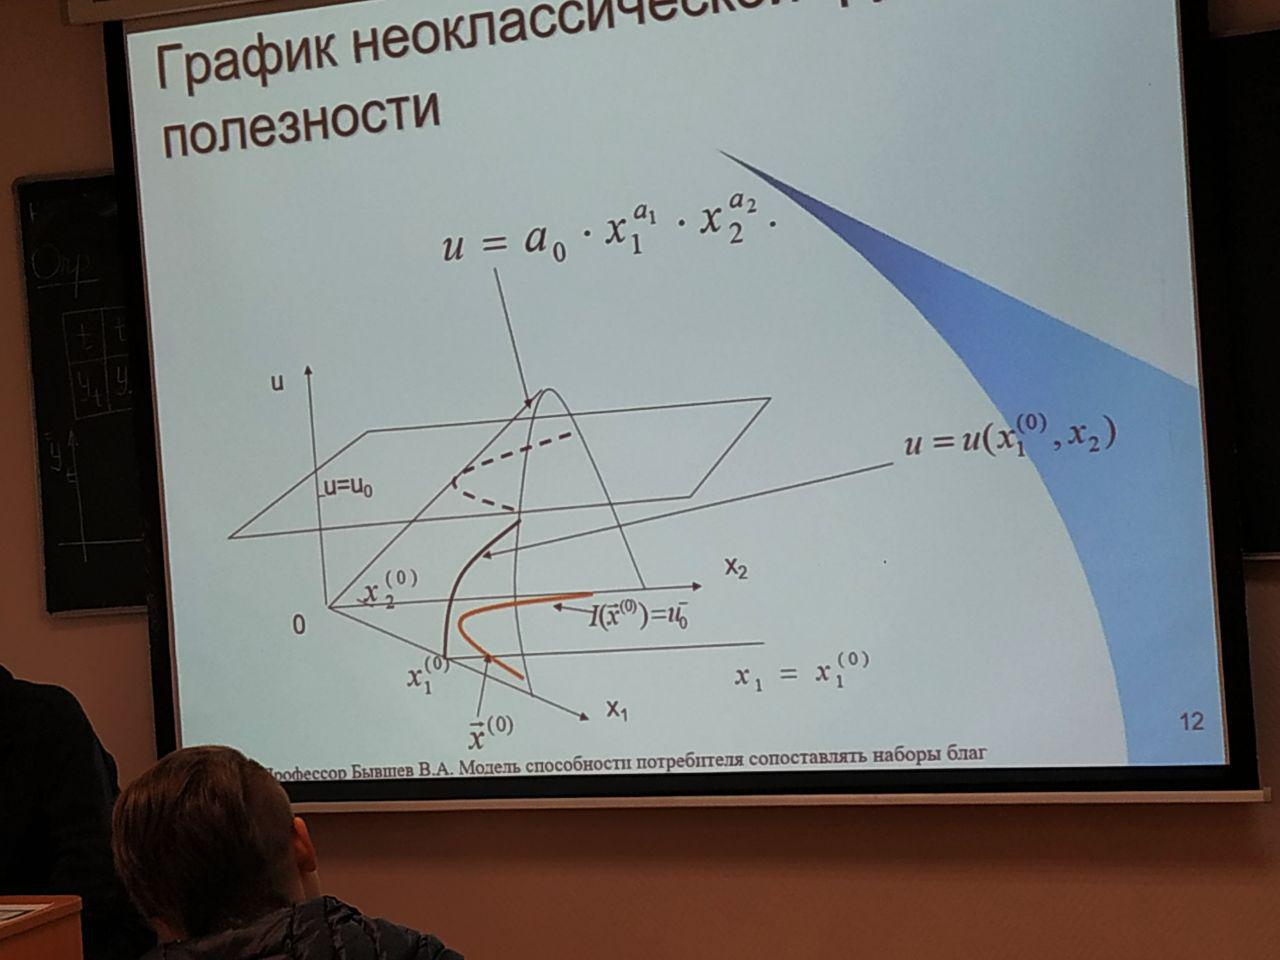
\includegraphics[width=0.5\textwidth]{img/photo_2019-09-26_16-41-58.jpg}
\end{figure}
\end{center}

На плоскости $\displaystyle x^{( 0)}$ мы обозначаем кирпичным цветом кривая безразличия. Точки которой, как набора благ имеют туже полезность, что и $\displaystyle \vec{x}_{0}$. Кривую безразличия мы можем обозначить $\displaystyle u^{-}_{0}$ прообразы.
\begin{center}
\textbf{Предельная полезности блага и закон Госсена}
\end{center}
Вернёмся к теореме Дебре; выпуклость вверхе функции полезности обозначает отрицательный знак второй производной по каждому аргументу:


\begin{equation*}
\frac{\partial ^{2} u}{\partial x^{2}_{i}} \ < \ 0 \eqno(9)
\end{equation*}


Проиллюстрируем на графике на примере двух благ:

\begin{center}
\begin{figure}[H]
  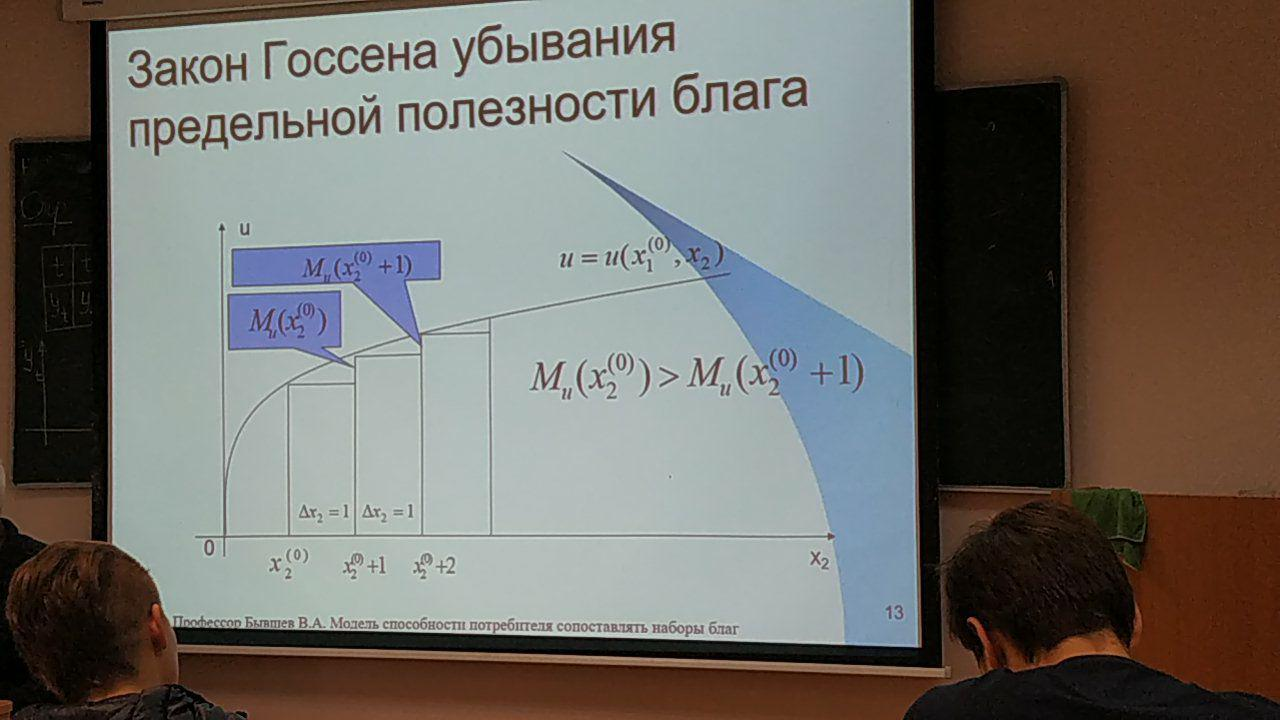
\includegraphics[width=0.5\textwidth]{img/photo_2019-09-26_16-52-14.jpg}
\end{figure}
\end{center}

\textbf{Закон Госсена.} Выпуклость вверх означает, что каждая следующая еденица блага приносит дополнительную полезность меньшую чем предыдущая дополнительная еденица. Это означает убывание предельной полезности любого блага при фиксированных значениях остальных благ.

Завершая лекцию дадим определение предельной полезности блага:
\begin{equation*}
\vartriangle u\ =\ M_{u}( x_{i}) \ =\ u( x_{1} ,\ \cdots ,\ x_{i} \ +\ 1,\ \cdots ,\ x_{n}) \ -\ u\ ( x_{1} ,\ \cdots ,\ x_{i} ,\ \cdots ,\ x_{n}) \  >0 \eqno(10)
\end{equation*}
Согласно теоремы Дебре предельная полезность всегда положительна. Добавим, что с позиции математики предельная полезность - это приращение функции полезности в ответ на прирощении аргумента $\displaystyle x_{i}$. И поэтому предельную полезность удобно вычеслить по правилу: $\displaystyle M_{u}( x_{i}) \ =\ \frac{\partial u}{\partial x_{i}}$.
\end{document}
